\documentclass[mathserif,hyperref]{beamer}

\usepackage[spanish]{babel}
\usepackage[utf8]{inputenc}
\usepackage{amsmath}
\usepackage{array}
\usepackage{caption}
\usepackage{adjustbox}
\usepackage{lmodern}

\usetheme{Luebeck}
\usecolortheme[rgb={0.67,0.05,0}]{structure}
\usecolortheme{beaver}

% elimina las siguientes advertencias:
% LaTeX Font Warning: Font shape `OT1/cmss/m/n' in size <4> not available
% (Font)              size <5> substituted on input line 22.
% LaTeX Font Warning: Size substitutions with differences
% (Font)              up to 1.0pt have occurred.

\title{Prueba de oposición}
\author{Lucas Gabriel Vuotto}
\date{\today}


% Adicional intercala package{beamerthemeshadow}
%\usepackage{beamerthemeshadow}
%  causa que elementos que aparece en el futuro
%  escribe ligero
%\beamersetuncovermixins{\opaqueness<1>{25}}{\opaqueness<2->{15}}
% funciona por tablas tamb\'\i en cuando aplica teTeX$B!D(B
\begin{document}


\begin{frame}
\titlepage %portada
\end{frame}


\begin{frame}
\frametitle{Índice}
\tableofcontents
\end{frame}


\section{Entorno}

\subsection{Contexto}
\begin{frame}
\frametitle{Contexto}
Para este ejercicio, se asume que los alumnos tienen conocimientos sobre los
siguiente temas:
\begin{itemize}
  \item compuertas lógicas básicas
  \item operaciones con números binarios.
  \item diseño de circuitos combinatorios.
\end{itemize}

\vspace{0.5cm}
Se recomienda dar este ejercicio \textbf{a modo integratorio}, antes de
comenzar con circuitos secuenciales.
\end{frame}


\subsection{Objetivos}
\begin{frame}
\frametitle{Objetivos}
\begin{itemize}
  \item Repasar circuitos combinatorios, en particular, aritméticos.
  \item Mostrar cómo se realizan los circuitos en la vida real.
\end{itemize}
\end{frame}


\subsection{Justificación de la elección}
\begin{frame}
\frametitle{Justificación de la elección}
Se eligió este ejercicio por ser interesante en el sentido de que ayuda a
darle a los alumnos un vistazo de cómo se hacen las cosas en el mundo real.

\vspace{0.5cm}
También se lo eligió porque al menos se suele dar en clase el circuito del
\textit{sumador simple}, mas no su implementación con NANDs.
\end{frame}


\section{Ejercicio}

\begin{frame}
\frametitle{Enunciado}
\textbf{Ejercicio 11}
{\tiny Organización del Computador I - práctica 2 (lógica digital) - segundo
cuatrimestre del 2014.}
\begin{enumerate}
  \item Diseñar un \textit{sumador completo} de 1 bit usando sólo compuertas
  NAND.
  \item Suponiendo que todas las compuertas elementales tienen el mismo
  retardo \textit{(delay)} $t$, calcule el retardo total del circuito para
  producir todas sus señales de salida.
\end{enumerate}
\end{frame}


\begin{frame}
\frametitle{\small Diseñar un \textit{sumador completo} de 1 bit usando sólo
compuertas NAND}
Tablas de verdad
\begin{columns}
  \column{.5\textwidth}
    \pause
    \begin{center}\begin{table}
    \begin{tabular}{| c | c || c | c |}
      \hline
      $e_0$ & $e_1$ & $c$ & $s$ \\ \hline
        0   &   0   &  0  &  0  \\
        0   &   1   &  0  &  1  \\
        1   &   0   &  0  &  1  \\
        1   &   1   &  1  &  0  \\
      \hline
    \end{tabular}
    \caption*{Sumador simple}
    \end{table}\end{center}
  \column{.5\textwidth}
    \pause
    \begin{center}\begin{table}
    \begin{tabular}{| c | c | c || c | c |}
      \hline
      $e_0$ & $e_1$ & $c_e$ & $s$ & $c_s$ \\ \hline
        0   &   0   &   0   &  0  &   0   \\
        0   &   1   &   0   &  0  &   1   \\
        1   &   0   &   0   &  0  &   1   \\
        1   &   1   &   0   &  1  &   0   \\
        0   &   0   &   1   &  0  &   1   \\
        0   &   1   &   1   &  1  &   0   \\
        1   &   0   &   1   &  1  &   0   \\
        1   &   1   &   1   &  1  &   1   \\
      \hline
    \end{tabular}
    \caption*{Sumador completo}
    \end{table}\end{center}
\end{columns}
\end{frame}


\begin{frame}
\frametitle{\small Diseñar un \textit{sumador completo} de 1 bit usando sólo
compuertas NAND}
\begin{figure}[htp]
  \caption{Sumador simple}
  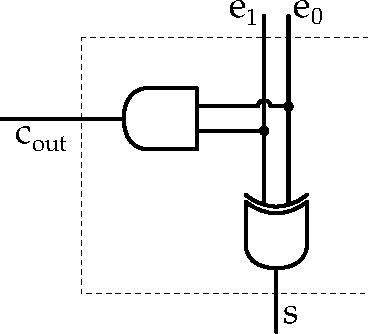
\includegraphics[scale=0.9]{sumador-simple.pdf}
\end{figure}
\end{frame}


\begin{frame}
\frametitle{\small Diseñar un \textit{sumador completo} de 1 bit usando sólo
compuertas NAND}
\begin{figure}[htp]
  \caption{Sumador completo}
  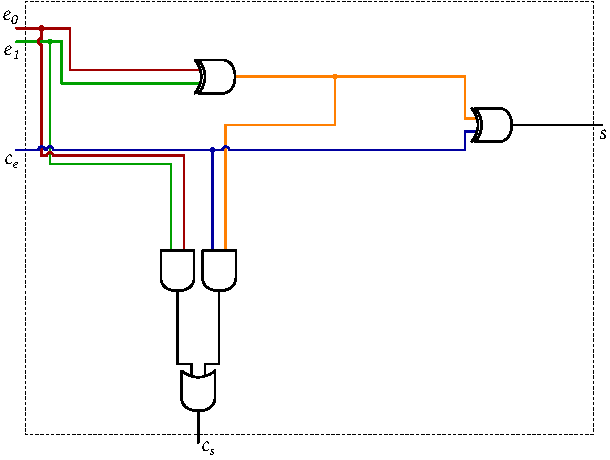
\includegraphics[scale=0.9]{sumador-completo.pdf}
\end{figure}
\end{frame}


\begin{frame}
\frametitle{\small Diseñar un \textit{sumador completo} de 1 bit usando sólo
compuertas NAND}
Para los que no recuerdan, esto es la tabla de verdad de un NAND:
\begin{center}\begin{tabular}{| c | c || c |}
  \hline
  $e_0$ & $e_1$ & $e_0$ \texttt{NAND} $e_1$ \\ \hline
    0   &   0   &             1             \\
    0   &   1   &             1             \\
    1   &   0   &             1             \\
    1   &   1   &             0             \\
  \hline
\end{tabular}\end{center}
\end{frame}


\begin{frame}
\frametitle{\small Diseñar un \textit{sumador completo} de 1 bit usando sólo
compuertas NAND}
\begin{center}Método matemático\end{center}
\begin{align*}
  s   &= e_0 \oplus e_1 \oplus c_e \\
  c_s &= (e_0 . e_1) + (e_0 \oplus e_1) . c_e
\end{align*}
\pause
\begin{center}{\Large ¡Aburrido!}\end{center}
\end{frame}


\begin{frame}
\frametitle{\small Diseñar un \textit{sumador completo} de 1 bit usando sólo
compuertas NAND}
\begin{center}
  Método gráfico
  \\ {\tiny (sigue siendo medio matemático)}
\end{center}
\end{frame}


\begin{frame}
\frametitle{\small Diseñar un \textit{sumador completo} de 1 bit usando sólo
compuertas NAND}
\begin{center}AND\end{center}
\begin{align*}
  \onslide<1->{x | y &= \overline{x . y} \Rightarrow \\}
  \onslide<2->{x . y &= }
  \onslide<3->{\overline{\overline{x . y}} = }
  \onslide<4->{\overline{x | y}}
\end{align*}
\end{frame}


\begin{frame}
\frametitle{\small Diseñar un \textit{sumador completo} de 1 bit usando sólo
compuertas NAND}
\begin{center}OR\end{center}
\begin{align*}
  \onslide<1->{x | y &= \overline{x . y} = \bar{x} + \bar{y} \Rightarrow \\}
  \onslide<2->{\bar{x} | \bar{y} &=
               \overline{\bar{x} . \bar{y}} =
               \bar{\bar{x}} + \bar{\bar{y}} =
               x + y}
\end{align*}
\end{frame}


\begin{frame}
\frametitle{\small Diseñar un \textit{sumador completo} de 1 bit usando sólo
compuertas NAND}
\begin{center}XOR\end{center}
\begin{align*}
  \onslide<1->{x \oplus y &= (x + y) . (\bar{x} + \bar{y}) \\}
  \onslide<2->{ &= (\bar{x} | \bar{y}) . (x | y) \\}
  \onslide<3->{ &= \overline{(\bar{x} | \bar{y}) | (x | y)}}
\end{align*}
\end{frame}


\begin{frame}
\frametitle{\small Diseñar un \textit{sumador completo} de 1 bit usando sólo
compuertas NAND}
\begin{center}NOT\end{center}
\begin{align*}
  \onslide<1->{x &= x . x \Rightarrow }
  \onslide<2->{\bar{x} = \overline{x . x}}
  \onslide<3->{ = x | x}
\end{align*}
\end{frame}


\begin{frame}
\frametitle{\small Diseñar un \textit{sumador completo} de 1 bit usando sólo
compuertas NAND}
\begin{center}Resumen\end{center}
\only<1>{
\begin{align*}
  x . y &= \overline{x | y} \\
  x + y &= \bar{x} | \bar{y} \\
  x \oplus y &=  \overline{(\bar{x} | \bar{y}) | (x | y)} \\
  \bar{x} &= x | x
\end{align*}
}
\only<2>{
\begin{align*}
  x . y &= (x | y) | (x | y) \\
  x + y &= (x | x) | (y | y) \\
  x \oplus y &= [((x | x) | (y | y)) \ | \ (x | y)] \ | \ 
                [((x | x) | (y | y)) \ | \ (x | y)] \\
  \bar{x} &= x | x
\end{align*}
}
\end{frame}


\begin{frame}[t]
\frametitle{\small Diseñar un \textit{sumador completo} de 1 bit usando sólo
compuertas NAND}
\textit{Sumador simple}
\begin{columns}[T]
  \column{.3\textwidth}
  \begin{figure}[htp]
    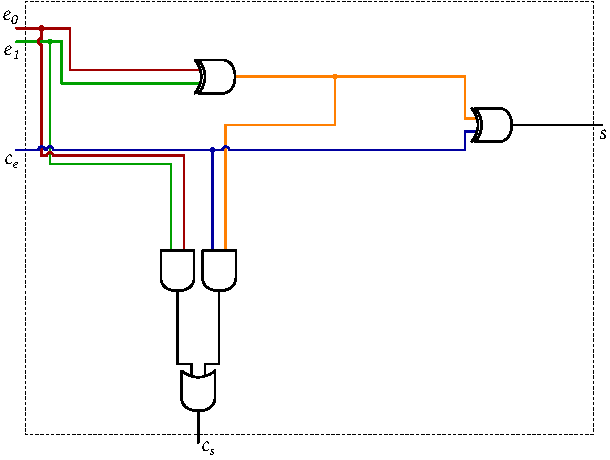
\includegraphics[scale=0.6]{sumador-completo.pdf}
  \end{figure}
  \column{.7\textwidth}
  \begin{center}\begin{tabular}{| c | c || c |}
    \hline
    $e_0$ & $e_1$ & $e_0$ \texttt{AND} $e_1$ \\ \hline
      0   &   0   &             0            \\
      0   &   1   &             0            \\
      1   &   0   &             0            \\
      1   &   1   &             1            \\
    \hline
  \end{tabular}\end{center}
  \pause
  \begin{center}\begin{tabular}{| c | c || c |}
    \hline
    $e_0$ & $e_1$ & $e_0$ \texttt{NAND} $e_1$ \\ \hline
      0   &   0   &              1            \\
      0   &   1   &              1            \\
      1   &   0   &              1            \\
      1   &   1   &              0            \\
    \hline
  \end{tabular}\end{center}
\end{columns}
\end{frame}


\begin{frame}[t]
\frametitle{\small Diseñar un \textit{sumador completo} de 1 bit usando sólo
compuertas NAND}
\textit{Sumador simple}
\begin{columns}[T]
  \column{.3\textwidth}
  \begin{figure}[htp]
    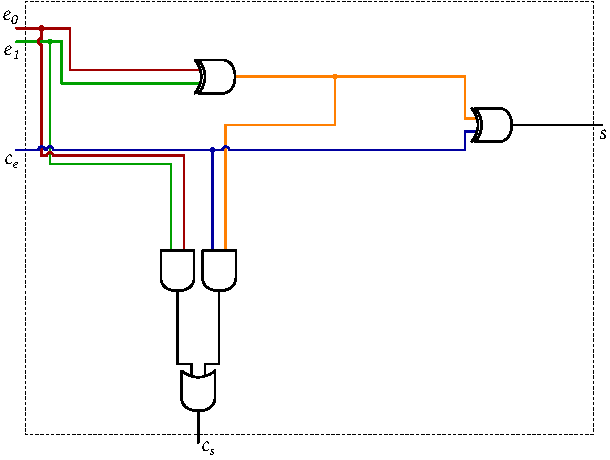
\includegraphics[scale=0.6]{sumador-completo.pdf}
  \end{figure}
  \column{.7\textwidth}
  \begin{center}\begin{tabular}{| c | c || c |}
    \hline
    $e$ & $1$ & NOT $e$ \\ \hline
     0  &  1  &    1    \\
     1  &  1  &    0    \\
    \hline
  \end{tabular}\end{center}
\end{columns}
\end{frame}


\begin{frame}[t]
\frametitle{\small Diseñar un \textit{sumador completo} de 1 bit usando sólo
compuertas NAND}
\textit{Sumador simple}
\begin{columns}[T]
  \column{.3\textwidth}
  \begin{figure}[htp]
    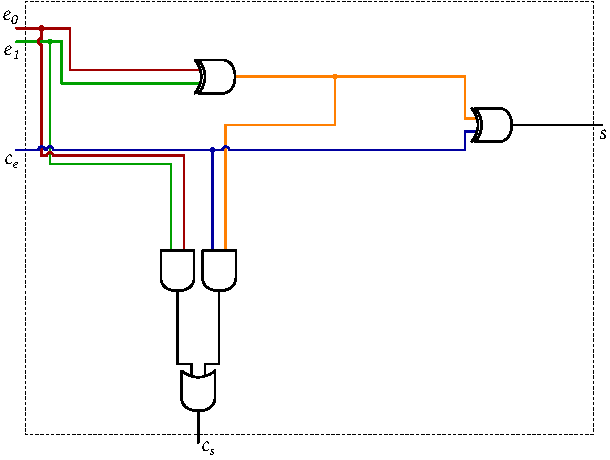
\includegraphics[scale=0.6]{sumador-completo.pdf}
  \end{figure}

  \column{.7\textwidth}
  \begin{center}
  \begin{tabular}{| c | c || c |}
    \hline
    $e_0$ & $e_1$ & $e_0$ NAND $e_1$ $(p)$ \\ \hline
      0   &   0   &            1           \\
      0   &   1   &            1           \\
      1   &   0   &            1           \\
      1   &   1   &            0           \\
    \hline
  \end{tabular}
  \pause
  \begin{tabular}{| c | c || c |}
    \hline
    $p$ & 1 & $p$ NAND 1 \\ \hline
     1  & 1 &      0     \\
     1  & 1 &      0     \\
     1  & 1 &      0     \\
     0  & 1 &      1     \\
    \hline
  \end{tabular}
  \end{center}
\end{columns}
% \\ ¡Grafiquito sumador simple en la derecha! updateamos la tablita del AND con
% la nueva info.
\end{frame}


\begin{frame}[t]
\frametitle{\small Diseñar un \textit{sumador completo} de 1 bit usando sólo
compuertas NAND}
\textit{Sumador simple}
\begin{columns}[T]
  \column{.3\textwidth}
  \begin{figure}[htp]
    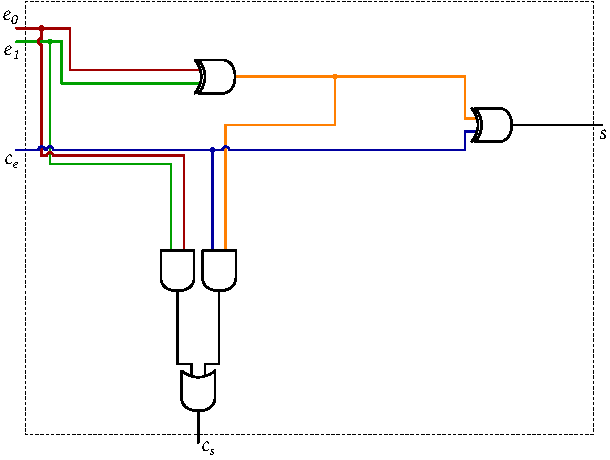
\includegraphics[scale=0.6]{sumador-completo.pdf}
  \end{figure}

  \column{.7\textwidth}
  \begin{center}\begin{tabular}{| c | c || c |}
    \hline
    $e_0$ & $e_1$ & $e_0$ OR $e_1$ \\ \hline
      0   &   0   &        0       \\
      0   &   1   &        1       \\
      1   &   0   &        1       \\
      1   &   1   &        1       \\
    \hline
  \end{tabular}\end{center}
  \pause
  \begin{center}\begin{tabular}{| c | c || c |}
    \hline
    $e_0$ & $e_1$ & $e_0$ NAND $e_1$ \\ \hline
      1   &   1   &         0        \\
      1   &   0   &         1        \\
      0   &   1   &         1        \\
      0   &   0   &         1        \\
    \hline
  \end{tabular}\end{center}
\end{columns}
% \\ ¡Grafiquito sumador simple en la derecha! ahora hacemos un OR con NANDs,
% pensandolo un poquito \textcolor{red}{$\Rightarrow$ \textbf{ARMAR LA IDEA}}.
\end{frame}


\begin{frame}[t]
\frametitle{\small Diseñar un \textit{sumador completo} de 1 bit usando sólo
compuertas NAND}
\textit{Sumador simple}
\begin{columns}[T]
  \column{.3\textwidth}
  \begin{figure}[htp]
    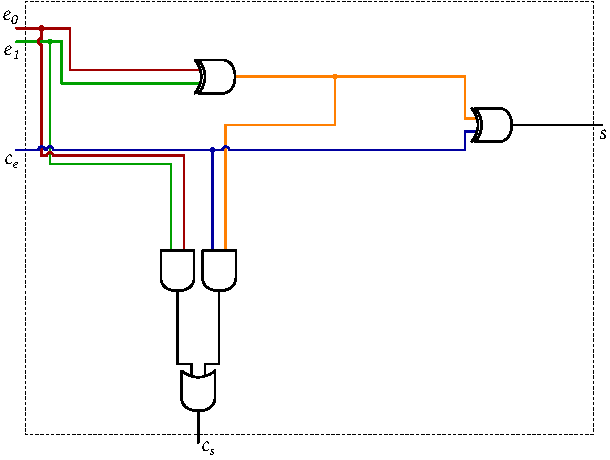
\includegraphics[scale=0.6]{sumador-completo.pdf}
  \end{figure}

  \column{.7\textwidth}
  Recordemos, $e_0$ XOR $e_1$ = ($e_0$ OR $e_1$) AND ($\lnot e_0$ OR $\lnot
  e_1$)
\end{columns}
% \\ ¡Grafiquito sumador simple en la derecha! cerramos haciendo un XOR con NANDs,
% también con alguna idea de cómo inferirlo.
\end{frame}


\begin{frame}[t]
\frametitle{\small Diseñar un \textit{sumador completo} de 1 bit usando sólo
compuertas NAND}
\textit{Sumador simple}
\begin{columns}[T]
  \column{.5\textwidth}
  \begin{figure}[htp]
    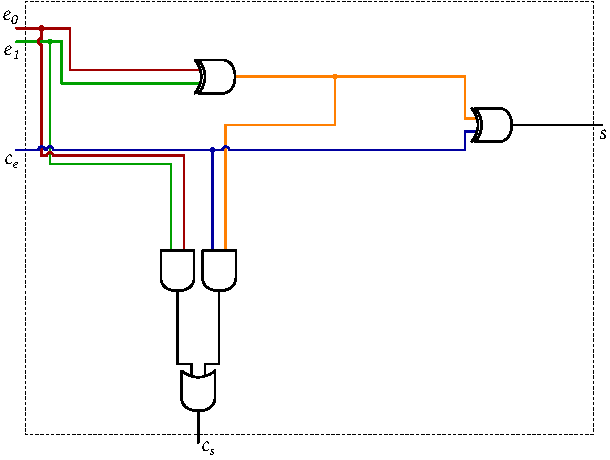
\includegraphics[scale=0.9]{sumador-completo.pdf}
  \end{figure}

  \column{.5\textwidth}
  \begin{figure}[htp]
    \includegraphics<1>[scale=0.9]{sumador-simple.pdf}
    \includegraphics<2>[scale=0.9]{sumador-completo.pdf}
  \end{figure}
\end{columns}
% \\ ¡Grafiquito sumador simple en la derecha! ahora vamos reemplazando en el
% grafico del sumador simple las compuertas AND, OR y XOR por sus equivalentes en
% NANDs.
\end{frame}


\begin{frame}[t]
\frametitle{\small Sabiendo que las compuertas elementales tienen un delay
de $t$, calcular el retardo total del circuito}
\begin{columns}
  \column{.5\textwidth}
  \begin{figure}[htp]
    \includegraphics<1-2>[scale=0.9]{sumador-completo.pdf}
    \includegraphics<3>[scale=0.6]{sumador-simple.pdf}
    \includegraphics<4->[scale=0.9]{sumador-completo.pdf}
  \end{figure}
  \pause
  \only<2>{$t + 2 (\text{sumador simple})$}
  \only<3>{$t + 2 (t + t)$}
  \only<4->{$t + 2 (2t) = 5t$}
  \column{.5\textwidth}
  
\end{columns}
\end{frame}


\begin{frame}
\begin{center}\Large ¿Preguntas?\end{center}
\end{frame}


\end{document}
